\documentclass[tikz]{standalone}
\usepackage[utf8x]{inputenc}
\usepackage{amsmath}
\usepackage{tikz}
\usetikzlibrary{arrows,matrix,positioning}
\begin{document}
    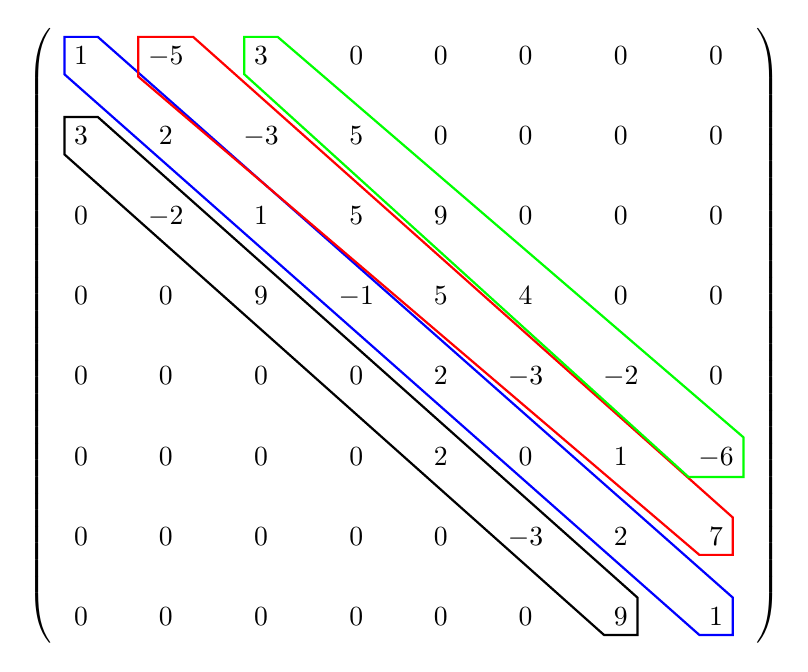
\begin{tikzpicture}
        \matrix [matrix of math nodes,left delimiter=(,right delimiter=), row sep=15pt, column sep = 15pt] (m)
        {
            1 & -5 & 3 & 0 & 0 & 0 & 0 & 0 \\
			3 & 2 & -3 & 5 & 0 & 0 & 0 & 0 \\
			0 & -2 & 1 & 5 & 9 & 0 & 0 & 0 \\
			0 & 0 & 9 & -1 & 5 & 4 & 0 & 0 \\
			0 & 0 & 0 & 0 & 2 & -3 & -2 & 0 \\
			0 & 0 & 0 & 0 & 2 & 0 & 1 & -6 \\
			0 & 0 & 0 & 0 & 0 & -3 & 2 & 7 \\
			0 & 0 & 0 & 0 & 0 & 0 & 9 & 1 \\
        };  
        \draw [color = blue, thick] (m-1-1.north west) -- (m-1-1.south west) -- (m-8-8.south west) -- (m-8-8.south east) -- (m-8-8.north east) -- (m-1-1.north east) -- cycle;
        \draw [color = black, thick] (m-2-1.north west) -- (m-2-1.south west) -- (m-8-7.south west) -- (m-8-7.south east) -- (m-8-7.north east) -- (m-2-1.north east) -- cycle;
        \draw [color = red, thick] (m-1-2.north west) -- (m-1-2.south west) -- (m-7-8.south west) -- (m-7-8.south east) -- (m-7-8.north east) -- (m-1-2.north east) -- cycle;
        \draw [color = green, thick] (m-1-3.north west) -- (m-1-3.south west) -- (m-6-8.south west) -- (m-6-8.south east) -- (m-6-8.north east) -- (m-1-3.north east) -- cycle;
    \end{tikzpicture}
\end{document}